% *********************************************************************
% © 2021-2023 Jeremy Sylvestre
%
% Permission is granted to copy, distribute and/or modify this document
% under the terms of the GNU Free Documentation License, Version 1.3 or
% any later version published by the Free Software Foundation; with no
% Invariant Sections, no Front-Cover Texts, and no Back-Cover Texts. A
% copy of the license is included in the appendix entitled “GNU Free
% Documentation License” that appears in the output document of this
% PreTeXt source code. All trademarks™ are the registered® marks of
% their respective owners.
%
% *********************************************************************

\newcommand*{\xmin}{-0.25}
\newcommand*{\xmax}{6.75}
\newcommand*{\ymin}{-1.5}
\newcommand*{\ymax}{1.5}

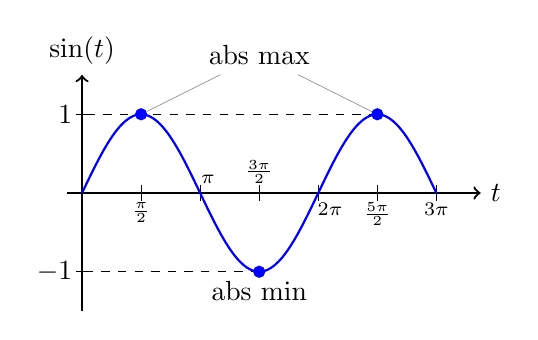
\begin{tikzpicture}
[
	closedpt/.style={circle,draw,fill,inner sep=0pt,minimum size=4pt},
	openpt/.style={circle,draw,inner sep=0pt,minimum size=4pt},
	xscale=0.75
]

	% axes
	\draw[->,thick] (\xmin,0) -- (\xmax,0) node[right] {$t$};
	\draw[->,thick] (0,\ymin) -- (0,\ymax) node[above] {$\sin(t)$};

	\foreach \x in {1,2,3,...,6} {
		\draw (\x,0.1) -- (\x,-0.1);
	}

	\node[below] at (1,0) {$\scriptstyle \frac{\pi}{2}$};
	\node[above,xshift=0.1cm] at (2,0) {$\scriptstyle \pi$};
	\node[above] at (3,0) {$\scriptstyle \frac{3 \pi}{2}$};
	\node[below,xshift=0.15cm] at (4,0) {$\scriptstyle 2 \pi$};
	\node[below] at (5,0) {$\scriptstyle \frac{5 \pi}{2}$};
	\node[below] at (6,0) {$\scriptstyle 3 \pi$};

	\draw[dashed] (5,1) -- (0,1) node[left] {$1$};
	\draw[dashed] (3,-1) -- (0,-1) node[left] {$-1$};
	\foreach \y in {-1,1} {
		\draw (-0.1,\y) -- (0.1,\y);
	}

	\node[blue,closedpt] at (1,1) (max1) {};
	\node[blue,closedpt] at (5,1) (max2) {};

	\node at (3,1.75) (maxlabel) {abs max};
	\draw[very thin, gray] (maxlabel) -- (max1);
	\draw[very thin, gray] (maxlabel) -- (max2);

	\node[blue,closedpt] at (3,-1) {};
	\node[below] at (3,-1) {abs min};

	\draw[blue,thick]
	  (0,0)
	  sin (1,1)
	  cos (2,0)
	  sin (3,-1)
	  cos (4,0)
	  sin (5,1)
	  cos (6,0)
	;

\end{tikzpicture}
